%% ============================================================
%% Teil II: rclcpp – ROS2 mit C++ (Kapitel 5–8)
%% Band 3 – Kapitel 5 bis 8
%% ============================================================

\part{rclcpp -- ROS2 mit C++}

% ─────────────────────────────────────────────────────────────
\chapter{Wir wollen einen C++-Node schreiben –
  rclcpp-Grundstruktur}
% ─────────────────────────────────────────────────────────────

\begin{lernziele}
Du schreibst den ersten rclcpp-Node mit CMakeLists.txt,
package.xml und \texttt{main()}-Funktion
und kannst den Unterschied zu rclpy erklären.
\end{lernziele}

\section{Situation}

Band~2 hat \texttt{arduino\_bridge\_node.py} mit rclpy gebaut.
Jetzt bauen wir \texttt{motor\_node.cpp} mit rclcpp --
die C++-Entsprechung.

\begin{aufgabeBox}
Schreibe \texttt{motor\_node.cpp} als minimalen rclcpp-Node,
trage ihn in \texttt{CMakeLists.txt} ein und starte ihn.
\end{aufgabeBox}

\section{Minimaler rclcpp-Node}

\begin{lstlisting}[style=cpp]
// src/motor_node.cpp -- Version 0.1
#include <rclcpp/rclcpp.hpp>

class MotorNode : public rclcpp::Node {
public:
    MotorNode() : Node("motor") {
        RCLCPP_INFO(this->get_logger(), "MotorNode gestartet.");
        timer_ = this->create_wall_timer(
            std::chrono::seconds(1),
            [this]() {
                RCLCPP_INFO(this->get_logger(), "Heartbeat");
            });
    }

private:
    rclcpp::TimerBase::SharedPtr timer_;
};

int main(int argc, char* argv[]) {
    rclcpp::init(argc, argv);
    auto node = std::make_shared<MotorNode>();
    rclcpp::spin(node);
    rclcpp::shutdown();
    return 0;
}
\end{lstlisting}

\begin{wissenBox}
\textbf{rclpy vs. rclcpp -- Vergleich}
\begin{center}
\begin{tabular}{lll}
\hline
\textbf{} & \textbf{rclpy (Band 2)} & \textbf{rclcpp (Band 3)} \\
\hline
Klasse & \texttt{class Node(Node):} & \texttt{class Node : public rclcpp::Node} \\
Konstruktor & \texttt{super().\_\_init\_\_("name")} & \texttt{: Node("name")} \\
Logger & \texttt{self.get\_logger().info()} & \texttt{RCLCPP\_INFO(logger, ...)} \\
Timer & \texttt{create\_timer(sek, cb)} & \texttt{create\_wall\_timer(chrono, cb)} \\
Init & \texttt{rclpy.init()} & \texttt{rclcpp::init(argc, argv)} \\
Spin & \texttt{rclpy.spin(node)} & \texttt{rclcpp::spin(node)} \\
Node-Ptr & Python-Objekt & \texttt{std::make\_shared<Node>()} \\
\hline
\end{tabular}
\end{center}
\end{wissenBox}

\begin{lstlisting}[style=cmake]
# CMakeLists.txt -- motor_node eintragen
add_executable(motor_node src/motor_node.cpp)
ament_target_dependencies(motor_node
    rclcpp geometry_msgs std_srvs)
install(TARGETS motor_node
    DESTINATION lib/${PROJECT_NAME})
\end{lstlisting}

\begin{lstlisting}[language=bash]
colcon build --packages-select robotik_uno_q_cpp
source install/setup.bash
ros2 run robotik_uno_q_cpp motor_node
# [INFO] [motor]: MotorNode gestartet.
# [INFO] [motor]: Heartbeat
\end{lstlisting}

\begin{projektBox}[robotik-uno-q -- Projektstand]
\textbf{Heute:} \texttt{motor\_node} als C++ kompiliert und gestartet.\\
\textbf{Nächstes Kapitel:} Subscriber für \texttt{/cmd\_vel}.
\end{projektBox}

\begin{merksatzBox}
\textbf{Merksatz:}
\texttt{RCLCPP\_INFO(get\_logger(), "...")} statt Python's \texttt{self.get\_logger().info()}.
\texttt{create\_wall\_timer(std::chrono::milliseconds(100), lambda)} für 10\,Hz.
\texttt{make\_shared<MotorNode>()} statt direktem Objekt.
\end{merksatzBox}

\begin{fehlerBox}
\begin{itemize}
\item \texttt{rclcpp::init()} vergessen: Segmentation Fault beim ersten
  \texttt{get\_logger()}-Aufruf.
\item Lambda mit \texttt{[]} statt \texttt{[this]}:
  \texttt{this->timer\_} nicht erreichbar im Callback.
\item \texttt{timer\_} nicht als Member gespeichert:
  Timer wird sofort zerstört, Callbacks feuern nie.
\end{itemize}
\end{fehlerBox}


% ─────────────────────────────────────────────────────────────
\chapter{Wir wollen \texttt{/cmd\_vel} empfangen –
  Subscriber in rclcpp}
% ─────────────────────────────────────────────────────────────

\begin{lernziele}
Du implementierst den \texttt{/cmd\_vel}-Subscriber im C++ \texttt{motor\_node}
und verstehst QoS-Profile in rclcpp.
\end{lernziele}

\section{Situation}

\texttt{navigation\_node.py} published \texttt{/cmd\_vel}.
\texttt{motor\_node.cpp} soll empfangen und den Arduino ansteuern.
Beide Nodes -- Python und C++ -- kommunizieren über das gleiche Topic.

\begin{aufgabeBox}
Füge dem \texttt{motor\_node.cpp} einen \texttt{/cmd\_vel}-Subscriber hinzu,
der bei jeder Nachricht Serial-Befehle an den Arduino sendet.
\end{aufgabeBox}

\section{Subscriber implementieren}

\begin{lstlisting}[style=cpp]
#include <rclcpp/rclcpp.hpp>
#include <geometry_msgs/msg/twist.hpp>

using Twist = geometry_msgs::msg::Twist;

class MotorNode : public rclcpp::Node {
public:
    MotorNode() : Node("motor") {
        // QoS: kompatibel mit navigation_node.py (RELIABLE, depth=10)
        auto qos = rclcpp::QoS(10).reliable();

        sub_cmd_ = this->create_subscription<Twist>(
            "/cmd_vel", qos,
            [this](const Twist::SharedPtr msg) {
                this->_verarbeite_twist(msg);
            });

        RCLCPP_INFO(get_logger(), "MotorNode: warte auf /cmd_vel ...");
    }

private:
    rclcpp::Subscription<Twist>::SharedPtr sub_cmd_;

    void _verarbeite_twist(const Twist::SharedPtr& msg) {
        float vx  = static_cast<float>(msg->linear.x);
        float wz  = static_cast<float>(msg->angular.z);

        // Differentialantrieb: Geschwindigkeit -> PWM-Werte
        // v_l = vx - (L/2)*wz,  v_r = vx + (L/2)*wz
        constexpr float SPURBREITE = 0.165f;  // Meter
        float v_r = vx + (SPURBREITE / 2.0f) * wz;
        float v_l = vx - (SPURBREITE / 2.0f) * wz;

        // Normieren auf [-1, 1], dann auf PWM [0, 255]
        // (vereinfacht: linearer Maßstab)
        constexpr float VMAX = 0.5f;
        int pwm_r = static_cast<int>(std::clamp(v_r / VMAX, -1.0f, 1.0f) * 255.0f);
        int pwm_l = static_cast<int>(std::clamp(v_l / VMAX, -1.0f, 1.0f) * 255.0f);

        _sende_serial(pwm_r, pwm_l);

        RCLCPP_DEBUG(get_logger(),
            "cmd_vel: vx=%.2f wz=%.2f -> R=%d L=%d", vx, wz, pwm_r, pwm_l);
    }

    void _sende_serial(int pwm_r, int pwm_l) {
        // Hier: Serial-Befehl senden (Kap. 12 vervollständigt das)
        // Format aus Band 1: "V 150 150\n"
        RCLCPP_INFO(get_logger(), "Sende: V %d %d", pwm_r, pwm_l);
    }
};
\end{lstlisting}

\begin{haubeBox}
\textbf{Differentialantrieb -- Kinematik in C++}

Die Kinematik des Differentialantriebs:
\[
v_r = v_x + \frac{L}{2} \cdot \omega_z, \quad
v_l = v_x - \frac{L}{2} \cdot \omega_z
\]
mit Spurbreite $L = 0{,}165$\,m, Translationsgeschwindigkeit $v_x$
und Rotationsrate $\omega_z$.

In Band~6 (Mathematik~I) werden diese Gleichungen formal hergeleitet.
Hier reicht die direkte Implementierung.
\end{haubeBox}

\begin{projektBox}[robotik-uno-q -- Projektstand]
\textbf{Heute:} C++ \texttt{motor\_node} empfängt \texttt{/cmd\_vel}
von Python \texttt{navigation\_node} -- Mix funktioniert.\\
\textbf{Nächstes Kapitel:} Lifecycle Nodes -- State Machine für robuste Motorsteuerung.
\end{projektBox}

\begin{merksatzBox}
\textbf{Merksatz:}
\texttt{create\_subscription<T>(topic, qos, lambda)} mit \texttt{T::SharedPtr} im Callback.
QoS muss kompatibel zum Publisher sein --
RELIABLE-Publisher + BEST\_EFFORT-Subscriber ergibt keine Verbindung.
\texttt{std::clamp(wert, min, max)} für sichere Wertebereichsbegrenzung.
\end{merksatzBox}


% ─────────────────────────────────────────────────────────────
\chapter{Wir wollen einen sicheren Motor-Node –
  Lifecycle Nodes in rclcpp}
% ─────────────────────────────────────────────────────────────

\begin{lernziele}
Du implementierst \texttt{motor\_node} als rclcpp Lifecycle~Node,
verstehst die State Machine (unconfigured/inactive/active/finalized)
und weißt, warum Lifecycle~Nodes für sicherheitskritische Hardware unverzichtbar sind.
\end{lernziele}

\section{Situation}

Ein normaler Node fährt sofort los.
Beim \texttt{motor\_node} ist das gefährlich:
Der Node darf die Motoren erst ansteuern,
wenn der Serial-Port offen, der Arduino bereit
und der Operateur bestätigt hat.

Lifecycle~Nodes lösen das: configure → activate → (Motor läuft) → deactivate.

\begin{aufgabeBox}
Konvertiere \texttt{motor\_node.cpp} zu einem
\texttt{rclcpp\_lifecycle::LifecycleNode}
mit korrekten Transitionen.
\end{aufgabeBox}

\section{Die Lifecycle-State-Machine}

\begin{center}
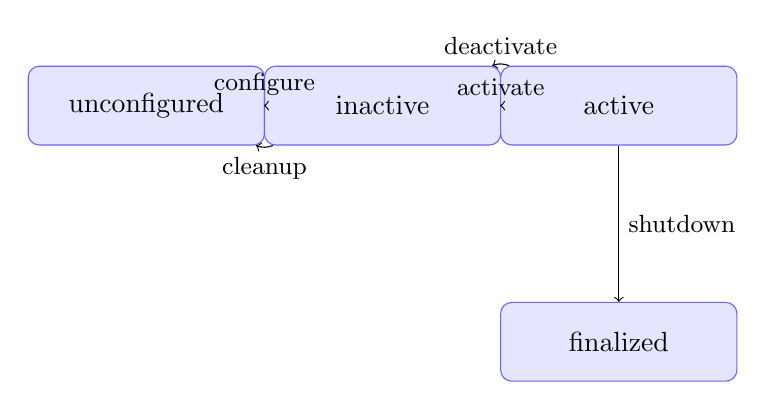
\begin{tikzpicture}[node distance=3cm, auto,
    state/.style={rectangle, rounded corners, draw=blue!60, fill=blue!10,
                  minimum width=3cm, minimum height=1cm}]
  \node[state] (unc)  {unconfigured};
  \node[state, right of=unc]  (ina)  {inactive};
  \node[state, right of=ina]  (act)  {active};
  \node[state, below of=act]  (fin)  {finalized};
  \draw[->] (unc) -- node[above]{\small configure} (ina);
  \draw[->] (ina) -- node[above]{\small activate}  (act);
  \draw[->] (act) -- node[right]{\small shutdown}  (fin);
  \draw[->] (ina) to[bend left=20] node[below]{\small cleanup} (unc);
  \draw[->] (act) to[bend right=20] node[above]{\small deactivate} (ina);
\end{tikzpicture}
\end{center}

\begin{lstlisting}[style=cpp]
#include <rclcpp_lifecycle/lifecycle_node.hpp>
#include <rclcpp_lifecycle/lifecycle_publisher.hpp>

using CallbackReturn = rclcpp_lifecycle::node_interfaces::LifecycleNodeInterface::CallbackReturn;

class MotorNode : public rclcpp_lifecycle::LifecycleNode {
public:
    MotorNode() : LifecycleNode("motor") {}

    // ── configure: Ressourcen allozieren, Serial öffnen ──────────────────
    CallbackReturn on_configure(const rclcpp_lifecycle::State&) override {
        RCLCPP_INFO(get_logger(), "Konfiguriere: Serial-Port öffnen...");
        try {
            serial_ = std::make_unique<SerialPort>("/dev/arduino", 9600);
            sub_cmd_ = this->create_subscription<geometry_msgs::msg::Twist>(
                "/cmd_vel", 10,
                [this](const geometry_msgs::msg::Twist::SharedPtr msg) {
                    this->_verarbeite_twist(msg);
                });
            RCLCPP_INFO(get_logger(), "Konfiguriert.");
            return CallbackReturn::SUCCESS;
        } catch (const std::exception& e) {
            RCLCPP_ERROR(get_logger(), "Konfiguration fehlgeschlagen: %s", e.what());
            return CallbackReturn::FAILURE;
        }
    }

    // ── activate: Motoren freigeben ───────────────────────────────────────
    CallbackReturn on_activate(const rclcpp_lifecycle::State&) override {
        RCLCPP_INFO(get_logger(), "Aktiviert: Motoren bereit.");
        motoren_aktiv_ = true;
        return CallbackReturn::SUCCESS;
    }

    // ── deactivate: Motoren stoppen, Subscriber bleibt ───────────────────
    CallbackReturn on_deactivate(const rclcpp_lifecycle::State&) override {
        motoren_aktiv_ = false;
        if (serial_) {
            serial_->sende("S\n");   // Stopp-Befehl
        }
        RCLCPP_INFO(get_logger(), "Deaktiviert: Motoren gestoppt.");
        return CallbackReturn::SUCCESS;
    }

    // ── cleanup: Ressourcen freigeben ─────────────────────────────────────
    CallbackReturn on_cleanup(const rclcpp_lifecycle::State&) override {
        sub_cmd_.reset();
        serial_.reset();
        RCLCPP_INFO(get_logger(), "Bereinigt.");
        return CallbackReturn::SUCCESS;
    }

private:
    std::unique_ptr<SerialPort> serial_;
    rclcpp::Subscription<geometry_msgs::msg::Twist>::SharedPtr sub_cmd_;
    std::atomic<bool> motoren_aktiv_{false};

    void _verarbeite_twist(const geometry_msgs::msg::Twist::SharedPtr& msg) {
        if (!motoren_aktiv_.load()) return;   // Sicherheitsprüfung
        // ... PWM berechnen und senden ...
    }
};
\end{lstlisting}

\begin{lstlisting}[language=bash]
# Lifecycle-Node starten
ros2 run robotik_uno_q_cpp motor_node

# State-Übergänge extern auslösen
ros2 lifecycle set /motor configure
ros2 lifecycle set /motor activate
ros2 lifecycle set /motor deactivate
ros2 lifecycle get /motor  # zeigt aktuellen State
\end{lstlisting}

\begin{projektBox}[robotik-uno-q -- Projektstand]
\textbf{Heute:} \texttt{motor\_node} als Lifecycle-Node.
Motoren starten erst nach explizitem \texttt{activate}.\\
\textbf{Nächstes Kapitel:} Services in C++ -- /motor/stopp als C++-Service.
\end{projektBox}

\begin{merksatzBox}
\textbf{Merksatz:}
\texttt{on\_configure}: Ressourcen allozieren, Subscriber erstellen.
\texttt{on\_activate}: Hardware freigeben.
\texttt{on\_deactivate}: Hardware sicher stoppen, Ressourcen behalten.
\texttt{on\_cleanup}: Ressourcen freigeben.
\texttt{CallbackReturn::SUCCESS} oder \texttt{FAILURE} -- kein throw.
\end{merksatzBox}


% ─────────────────────────────────────────────────────────────
\chapter{Wir wollen eine Notbremse in C++ –
  Services in rclcpp}
% ─────────────────────────────────────────────────────────────

\begin{lernziele}
Du implementierst \texttt{/motor/stopp} als \texttt{std\_srvs::srv::Trigger}-Service
in C++ und rufst ihn vom Python-\texttt{navigation\_node} aus auf.
\end{lernziele}

\section{Situation}

In Band~2 war \texttt{/motor/stopp} ein Python-Service.
Jetzt ist \texttt{motor\_node} in C++.
Der Service muss neu implementiert werden --
aber der Python-Client aus Band~2 soll weiter funktionieren,
denn ROS2-Services sind sprachunabhängig.

\begin{aufgabeBox}
Implementiere \texttt{/motor/stopp} als C++-Service-Server
und stelle sicher, dass der Python-Client aus Band~2 ihn aufruft.
\end{aufgabeBox}

\section{Service-Server in C++}

\begin{lstlisting}[style=cpp]
#include <std_srvs/srv/trigger.hpp>

using Trigger = std_srvs::srv::Trigger;

class MotorNode : public rclcpp_lifecycle::LifecycleNode {
public:
    MotorNode() : LifecycleNode("motor") {
        // Service schon im Konstruktor -- muss immer erreichbar sein
        srv_stopp_ = this->create_service<Trigger>(
            "/motor/stopp",
            [this](const Trigger::Request::SharedPtr req,
                         Trigger::Response::SharedPtr res) {
                this->_stopp_callback(req, res);
            });
        RCLCPP_INFO(get_logger(), "Service /motor/stopp bereit.");
    }

private:
    rclcpp::Service<Trigger>::SharedPtr srv_stopp_;

    void _stopp_callback(
        const Trigger::Request::SharedPtr&,
        Trigger::Response::SharedPtr& res)
    {
        RCLCPP_WARN(get_logger(), "NOTBREMSE ausgeloest!");
        motoren_aktiv_.store(false);

        try {
            if (serial_) {
                serial_->sende("S\n");
            }
            res->success = true;
            res->message = "Motoren gestoppt.";
        } catch (const std::exception& e) {
            res->success = false;
            res->message = std::string("Fehler: ") + e.what();
            RCLCPP_ERROR(get_logger(), "Stopp-Fehler: %s", e.what());
        }
    }
};
\end{lstlisting}

\begin{lstlisting}[language=bash]
# Testen: C++-Service von der Kommandozeile aufrufen
ros2 service call /motor/stopp std_srvs/srv/Trigger

# Python-Client aus Band 2 ruft C++-Service auf -- funktioniert unverändert
ros2 run robotik_uno_q navigation_node
\end{lstlisting}

\begin{projektBox}[robotik-uno-q -- Projektstand]
\textbf{Heute:} C++-Service-Server + Python-Client --
gemischter Stack funktioniert komplett.\\
\textbf{Teil~III:} Echtzeit und Performance.
\end{projektBox}

\begin{merksatzBox}
\textbf{Merksatz:}
Services in ROS2 sind sprachunabhängig --
C++-Server und Python-Client kommunizieren ohne Änderungen.
\texttt{create\_service<T>(name, lambda)} mit
\texttt{Request::SharedPtr} und \texttt{Response::SharedPtr}.
Exception im Service-Callback → \texttt{res->success = false}, nie propagieren.
\end{merksatzBox}
